\fig{fv:o1:critical}{改变同一入射光的角度，折射支路到临界角终止}{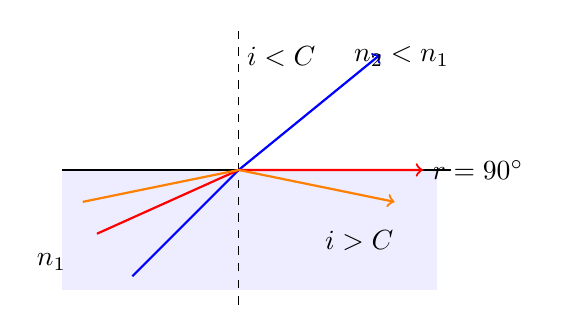
\begin{tikzpicture}[scale=.9]
\fill[blue!7](-2.5,-1.7)rectangle(2.8,0);\draw[thick](-2.5,0)--(3,0);
\draw[dashed](0,-1.9)--(0,2);\draw[->,blue,thick](-1.5,-1.5)--(0,0)--(2,1.63);
\draw[->,red,thick](-2,-.9)--(0,0)--(2.6,0);
\draw[->,orange,thick](-2.2,-.45)--(0,0)--(2.2,-.45);
\node[left]at(-2.3,-1.3){$n_1$};\node at(2.3,1.6){$n_2<n_1$};
\node[right]at(2.6,0){$r=90^\circ$};\node at(1.7,-1){$i>C$};\node at(.6,1.6){$i<C$};
\end{tikzpicture}}
在图\ref{fv:o1:critical}中，蓝光线有实数折射角；红光线沿界面，是 $\sin r=1$的边界；橙光线只保留反射支路。将 $i>C$代入 $n_1\sin i=n_2\sin r$会要求 $\sin r>1$，这表示传播折射支路不存在，不能继续对该值取反正弦。临界时的掠射光也不能当成进入上方介质并到达任意观察点的普通光路。
